\documentclass{beamer}
\usepackage{tikz}
\usepackage{lmodern}
\usepackage[orientation=landscape,size=a0,scale=2]{beamerposter}
\usepackage[absolute,overlay]{textpos}
\usetikzlibrary{shapes,arrows}
\usetikzlibrary{petri}
\usetikzlibrary{automata}

\begin{document}

\begin{textblock}{15}(0.5, 0.5)
    \begin{block}{}
        \centering
        \Large Suppression of Variation in Cell-Size: A Control Theoretic Approach \\
        \large Dilawar Singh, \texttt{dilawars@ncbs.res.in}
    \end{block}
    \begin{block}{Abstract}

        Building over a recent work \cite{paulsson}, we explored possibility of
        creating networks of small network which can be used to control cell
        size. We explored few network topologies of a simple control network
        which can keep the size of the cell at a fixed value while giving a
        upper bound on the size of the Endosome. We also wrote a skeleton for
        simulating these topologies in an event-driven simulation environment
        (SystemC library of C++) \cite{github}.

\end{block}
\end{textblock}

\begin{textblock}{7}(0.5,3.5)

    \begin{block}{Network under study}
        \begin{figure}
            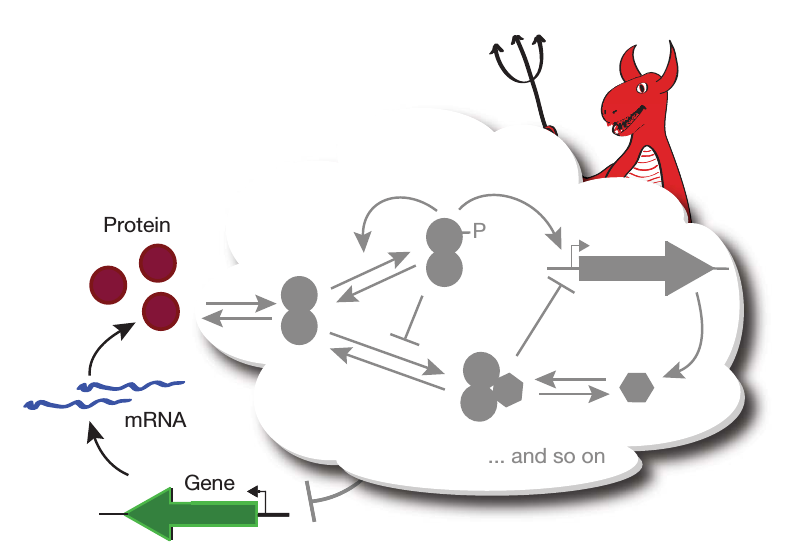
\includegraphics[scale=1]{./fig_mrna_protein.png}
            \begin{tikzpicture}[
                ]
            \node[place,tokens=1,label=above:$X_1$] (X1) at (0,0) {};
            \node[place,colored tokens={red,red,red},label=below:$X_2$] (X2) at (0,-5) {};

            \node[transition,minimum size=10mm,blue,fill,label=above:$f$] (birth) at (3,0) {};
            \node[transition,red,minimum size=10mm,fill,label=below:$\tau$] (death) at (3,-5) {};

            \node[place,label=above:Birth] (Xb) at (10,0) {$+1$};
            \node[place,label=below:Death] (Xd) at (10,-5) {$-1$};


            \draw[ultra thick,-triangle 90] (X1) to (birth) to (Xb);
            \draw[ultra thick,-triangle 90] (X1) to  (death);

            \draw[ultra thick,-triangle 90] (X2) to (death)  to (Xd);
            \draw[ultra thick,-triangle 90] (X2) to (birth);

            \draw[ultra thick,-triangle 90,blue] (Xb) to [bend right]  (birth);
            \draw[ultra thick,-triangle 90,blue] (Xb) to (death);

            \draw[ultra thick,red,-triangle 90] (Xd) to [bend left] (death) (Xd) to (birth);

            \end{tikzpicture} 
            
           
            
            \caption{\small On left, mRNA/Protein network. In
                our scheme $X_1$ is mRNA and $X_2$ is its protein. Genes are
                intermediate variables which are not shown in network.
                Intermediate variable appears only in feedback path. On right,
                an equivalent Petri net with some details omitted. }
            \label{fig:demon} \end{figure}



    \begin{eqnarray*}
        \tiny
            X_1 \xrightarrow{f'(x_2(-\infty,t))} X_1 + 1 \qquad X_1 \xrightarrow{\tau_{x_1}} X_1 -1 \\
            X_2 \xrightarrow{f(x_1)} X_2 + 1 \qquad X_2 \xrightarrow{\tau_{x_2}} X_2 - 1
    \end{eqnarray*}

   
    \end{block}

    \begin{block}{Information loss in this network}
        \begin{tikzpicture}[scale=1]
            % This one is information theory approach
            \tikzstyle{block} = [draw,rectangle, inner sep=15mm];

            \node (input) at (-10,0) {};
            \node (input_midway) at (-5,0) {};
            \node[block] (encoder) at (0,0) {Encoder};
            \node[block,right of=encoder,node distance=15 cm] (channel)  {Channel};
            \node[block,right of=channel,node distance=15 cm] (decoder)  {Decoder};
            \node[right of=decoder,node distance=10 cm] (output) {};
            \node[right of=decoder, node distance=7 cm] (output_mid) {};


            \draw[-triangle 90] (input) node[above] {$\xi$} -- (encoder);
            \draw[-triangle 90] (encoder) -- node[above] {$f(x_1)$} (channel);
            \draw[-triangle 90] (channel) -- node[above] {$x_2$} (decoder);
            \draw[-triangle 90] (decoder) --  node[above] {$\eta$} (output);

            \draw[-triangle 90] (output_mid) -| ++(0,-5) -- ++(-15,0) 
            node[above] {$f'(x_2(-\infty,0))$} -| (encoder);

        \end{tikzpicture}
        \def\mean#1{\left< #1 \right>}
        \begin{eqnarray}
            C = \mean{f} \log(1 + \frac{\sigma_f^2}{\mean{f}^2}
        \end{eqnarray}
    \end{block}

\end{textblock}

\begin{textblock}{7}(8,3.5)

    \begin{block}{The bounds}

        The following stochastic equation describes $x_1$.
        \def\mean#1{\left< #1 \right>}
        \begin{equation}
            dx_1 = (\frac{f'-x_1}{\tau _1}) dt + \sqrt{2\mean{x_1}/\tau_1}dw
        \end{equation}

        Following result \cite{paulsson} sets the bound on the variation on
        $x_1$ for the given optimal rate function $f'$ and any $\tau_2$.

        \begin{equation}
            \frac{\sigma_{x_1}^2}{\mean{x_1}} \geq \frac{1}{\sqrt{N_1N_2}}
        \end{equation}

    \end{block}
 
\end{textblock}

\end{document}
